\documentclass{standalone}
\usepackage{pgfplots}
\pgfplotsset{compat=1.15}
% Grouping the common style settings here to make the code below easier to read
\pgfkeys{/pgfplots/Axis Style/.style={
    width=13.5cm, height=5cm,
    axis x line=center, 
    axis y line=middle, 
    samples=100,
    ymin=-1.5, ymax=1.5,
    xmin=-7.0, xmax=7.0,
    domain=-2*pi:2*pi
}}

\begin{document}
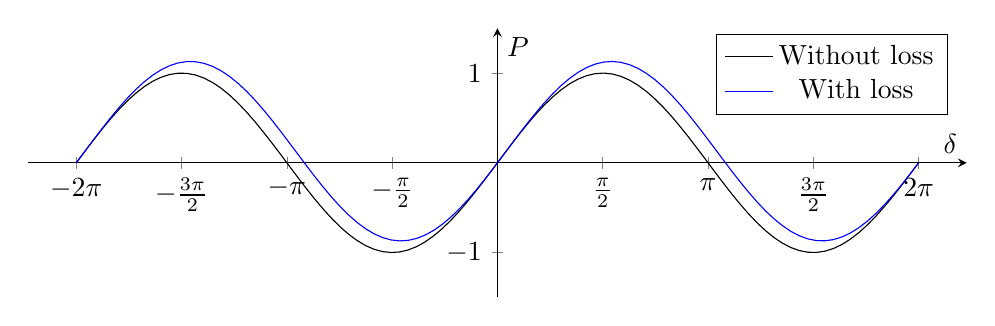
\begin{tikzpicture}
\begin{axis}[
    Axis Style,
    xtick={
        -6.28318, -4.7123889, -3.14159, -1.5708,
        1.5708, 3.14159, 4.7123889, 6.28318
    },
    xticklabels={
        $-2\pi$, $-\frac{3\pi}{2}$, $-\pi$, $-\frac{\pi}{2}$,
        $\frac{\pi}{2}$, $\pi$, $\frac{3\pi}{2}$, $2\pi$
    },
    xlabel={$\delta$},
    ylabel={$P$}
]
\addplot [mark=none, thin, black] {sin(deg(x))}
        %node[pos=.83, below] {Real power flow}
        ;
\addplot [mark=none, thin, blue] {sin(deg(x-0.13)) + sin(deg(0.13)}
         %node[pos=.63, above] {Real power flow}
         ;
\legend{Without loss, With loss}

\end{axis}
\end{tikzpicture}


\end{document}